%\documentclass[letterpaper, 10pt, conference]{ieeeconf}
\documentclass[12pt, reqno]{article} 
%\IEEEoverridecommandlockouts \overrideIEEEmargins
\usepackage[letterpaper, total={7.2in, 9.6in},tmargin=0.7in,lmargin=0.65in]{geometry}% mah
\usepackage{amsmath,amssymb,url}
\usepackage{graphicx,subfigure,warmread}
\usepackage[all,import]{xy}
\usepackage{color}
\usepackage{epstopdf}%
%\usepackage{scalerel,stackengine}
\usepackage{tikz}
\usetikzlibrary{shapes.geometric, arrows}
\usepackage{float}
\graphicspath{{./figures/}}% path to images


\newcommand{\norm}[1]{\ensuremath{\left\| #1 \right\|}}
\newcommand{\abs}[1]{\ensuremath{\left| #1 \right|}}
\newcommand{\bracket}[1]{\ensuremath{\left[ #1 \right]}}
\newcommand{\braces}[1]{\ensuremath{\left\{ #1 \right\}}}
\newcommand{\parenth}[1]{\ensuremath{\left( #1 \right)}}
\newcommand{\ip}[1]{\ensuremath{\langle #1 \rangle}}
\newcommand{\refeqn}[1]{(\ref{eqn:#1})}
\newcommand{\reffig}[1]{Fig. \ref{fig:#1}}
\newcommand{\tr}[1]{\mbox{tr}\ensuremath{\negthickspace\bracket{#1}}}
\newcommand{\deriv}[2]{\ensuremath{\frac{\partial #1}{\partial #2}}}
\newcommand{\G}{\ensuremath{\mathsf{G}}}
\newcommand{\SO}{\ensuremath{\mathsf{SO(3)}}}
\newcommand{\T}{\ensuremath{\mathsf{T}}}
\renewcommand{\L}{\ensuremath{\mathsf{L}}}
\newcommand{\so}{\ensuremath{\mathfrak{so}(3)}}
\newcommand{\SE}{\ensuremath{\mathsf{SE(3)}}}
\newcommand{\se}{\ensuremath{\mathfrak{se}(3)}}
\renewcommand{\Re}{\ensuremath{\mathbb{R}}}
\newcommand{\Sph}{\ensuremath{\mathsf{S}}}
\newcommand{\aSE}[2]{\ensuremath{\begin{bmatrix}#1&#2\\0&1\end{bmatrix}}}
\newcommand{\ase}[2]{\ensuremath{\begin{bmatrix}#1&#2\\0&0\end{bmatrix}}}
\newcommand{\D}{\ensuremath{\mathbf{D}}}
\newcommand{\pair}[1]{\ensuremath{\left\langle #1 \right\rangle}}
\newcommand{\met}[1]{\ensuremath{\langle\!\langle #1 \rangle\!\rangle}}
\newcommand{\Ad}{\ensuremath{\mathrm{Ad}}}
\newcommand{\ad}{\ensuremath{\mathrm{ad}}}
\newcommand{\g}{\ensuremath{\mathfrak{g}}}
\newcommand{\btheta}{\ensuremath{\boldsymbol\theta}}
\usepackage{hyperref}

\title{\LARGE \bf
Final expressions for Tiger 700 motor and 11*3.7 CF propeller with 14.8 V}

\author{Mahdis Bisheban}

\newcommand{\EditTL}[1]{{\color{red}\protect #1}}
\renewcommand{\EditTL}[1]{{\protect #1}}


\newtheorem{definition}{Definition}
\newtheorem{lem}{Lemma}
\newtheorem{prop}{Proposition}
\newtheorem{remark}{Remark}


\begin{document}
\allowdisplaybreaks
\maketitle \thispagestyle{empty} \pagestyle{empty}


The following is from experimental data:
\begin{gather}
      Throttle = p_1T^2 + p_2*T + p_3\\
      \text{Coefficients (with 95\% confidence bounds):}\\
        p_1 =      -1.784  (-2.176, -1.392)\\
        p_2 =       38.45  (34.62, 42.28)\\
        p_3 =       6.359  (-0.6873, 13.4)
\end{gather}


\begin{gather}
\tau =  p_1 T + p_2\\
\text{Coefficients (with 95\% confidence bounds):}\\
p_1 =     0.01351  (0.01283, 0.01419)\\
p_2 =    0.006128  (0.002816, 0.009441)\\
\end{gather}

The following is from motor manual:
\begin{gather}
\tau = p_1 T + p_2\\
\text{Coefficients (with 95\% confidence bounds):}\\
p_1 =     0.01719  (0.01498, 0.0194)\\
p_2 =    0.005421  (-0.01431, 0.02515)\\
\end{gather}

\begin{figure}[H]
	\centering
	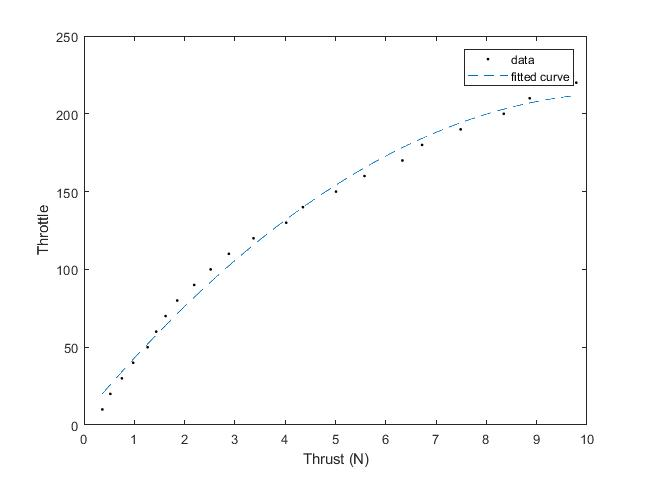
\includegraphics[width=0.4\columnwidth]{throttle_thrust}
	\caption{Throttle vs thrust (N)}\label{fig2}
\end{figure}

\begin{figure}[H]
	\centering
	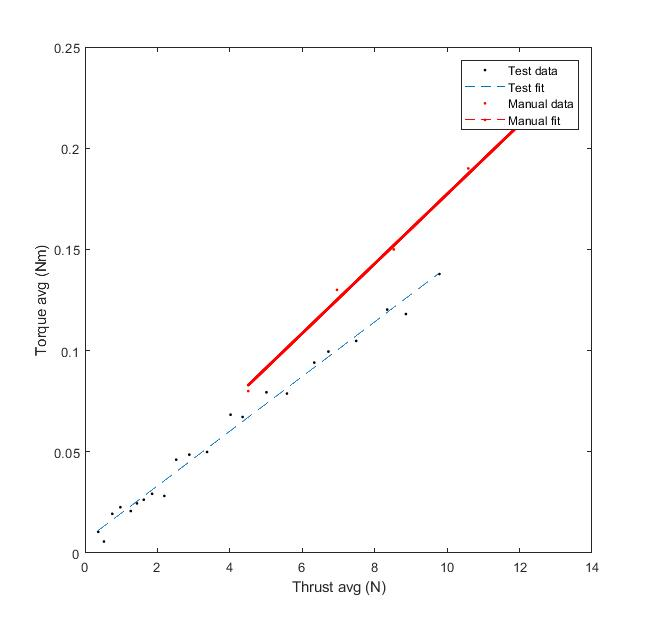
\includegraphics[width=0.4\columnwidth]{C_tau}
	\caption{Torque (Nm) vs thrust (N)}\label{fig1}
\end{figure}
%\begin{figure}[H]%
%\centerline{
%	\subfigure[Position]{\includegraphics[width=0.50\columnwidth]{X}}
%	\hfill
%	\subfigure[Velocity]{\includegraphics[width=0.50\columnwidth]{V}}	
%}
%\centerline{
%	\subfigure[Attitude]{\includegraphics[width=0.50\columnwidth]{R}}
%	\hfill
%	\subfigure[Angular velocity]{\includegraphics[width=0.50\columnwidth]{Omega}}	
%}
%\caption{Case I: Trajectories (The true and estimated plots are pretty close) $Red: estimated$, $Blue: initial$, $Cyan: true$. }
%\label{fig:traj}
%\end{figure}

\end{document}
